\documentclass[11pt]{article}
\usepackage[a4paper, portrait, margin=1in]{geometry}
\usepackage{listings}
\usepackage[dvipsnames]{xcolor}
\usepackage{color}
\usepackage{graphicx}
\usepackage[colorlinks=true,urlcolor=blue,linkcolor=gray]{hyperref}
% Fancy header package for version number

\usepackage{fancyhdr}
\pagestyle{fancy}
\fancyhf{}
\renewcommand{\headrulewidth}{0pt}
\renewcommand{\footrulewidth}{0pt}

\fancypagestyle{firstpagefooter}
{
\lfoot{Version: 29.09.2016}
\cfoot{}
\rfoot{\thepage}
}
\cfoot{\thepage}

\newcommand{\code}[1]{\lstinline[language=Java]{#1}}
\newcommand{\todo}[1]{\fcolorbox{black}{Apricot}{TODO: #1}}
\newcommand{\linkmain}[1]{\href{https://gitlab.inf.ethz.ch/pungast/asl-fall16-project/blob/master/src/main/java/asl/#1.java}{#1}}
\newcommand{\linktest}[1]{\href{https://gitlab.inf.ethz.ch/pungast/asl-fall16-project/blob/master/src/test/java/asl/#1.java}{#1}}

\begin{document}

\title{Advanced Systems Lab (Fall'16) -- First
Milestone}

\author{\textbf{Name: \emph{Your name}}\\\textbf{Legi number: \emph{Your legi
number}}}

\date{
\vspace{4cm}
\textbf{Grading} \\
\begin{tabular}{|c|c|}
\hline  \textbf{Section} & \textbf{Points} \\
\hline  1.1 &  \\ 
\hline  1.2 &  \\ 
\hline  1.3 &  \\ 
\hline  1.4 &  \\ 
\hline  2.1 &  \\ 
\hline  2.2 &  \\ 
\hline  3.1 &  \\ 
\hline  3.2 &  \\ 
\hline  3.3 &  \\ 
\hline \hline Total & \\
\hline 
\end{tabular} 
}

\maketitle
\thispagestyle{firstpagefooter}
\newpage

\section*{Notes on writing the report \small{(remove this page for submission)}}

The report for first milestone not need to be extensive but it must be concise, complete, and correct. 
Conciseness is important in terms of content and explanations, focusing on what has been done and explanations of the results. A long report is not necessarily a better report, especially if there are aspects of the design or the experiments that remain unexplained. Completeness implies that the report should give a comprehensive idea of what has been done by mentioning all key aspects of the design, experiments, and analysis. Aspects of the system, be it of its design or of its behavior, that remain unexplained detract from the credibility of the report. Correctness is expected in terms of the explanations being logical and correlate with the numbers in the experiments and the design.

Remember that this is a report about the system you have designed and built, about the experiments you have performed, and about how you interpret the results of the experiments and map them to your design and implementation. Please do not contact us seeking confirmation and assurances about, e.g., whether the report is sufficient, your interpretation of the data, validation of concrete aspects of your design, or whether you have done enough experiments. Making those decisions is your job and part of what the course will evaluate.

The report will be graded together with the code and data submitted. \textbf{The maximum number of points is 200 for each of the milestones and you will need at least 100 to pass. Keep in mind that to pass the project you need to collect at least 400 points from the three milestones.} You might be called for a meeting in person to clarify aspects of the report or the system and to make a short presentation of the work done. By submitting the report, the code, and the data, you confirm that you have done the work on your own, the code has been developed by yourself, the data submitted comes from experiments your have done, you have written the report on your own, and you have not copied neither code nor text nor data from other sources.

\medskip
\noindent
A passing grade for the milestone requires at the very minimum:
\begin{itemize}
\item Conforming to this template
\item A working system
\item Consistent experimental results of the entire system
\item Internal measurements of the middleware
\item Solid and credible explanations of the design, experimental results and behavior of the implemented system
\end{itemize}

\section*{Formatting guidelines}
We expect you to use this template for the report, but in case you want to use Word or an other text processor, keep in mind the following:
\begin{itemize}
\item  We expect you to submit \textbf{a single PDF that has the same section structure as this template, and answers all points we outline here}. If you use this file, you should remove this page with notes, and the short description provided by us at the beginning of sections.
\item Keep the same cover page as on this document and \textbf{fill out your name and legi number}. Leave the grading table empty.
\item  The main text should be in \textbf{single-column format with 11pt font on A4 paper}. In case you don't start with one of the files provided by us, \textbf{for margins use 2.54 cm (1 inch) on all sides}.
\end{itemize}


\section{System Description}\label{sec:system-description}

\subsection{Overall Architecture}\label{sec:desc:architecture}

The most important classes in this implementation all belong to the package \code{main.java.asl} and are as follows. Note that whenever a Java class is referenced, it will appear as a link to GitLab, e.g. \linkmain{MiddlewareMain}. 

\begin{itemize}
\item \linkmain{MiddlewareMain} is responsible for setting up all parts of the middleware.
\item \linkmain{Request} is a wrapper class for all GET- or SET-requests.
\item \linkmain{LoadBalancer} is the front of the middleware. It reads all incoming requests from all clients using \code{java.nio}, hashes the requests using a \linkmain{Hasher} and forwards them to the correct servers for writing or reading. When a request has a response, \linkmain{LoadBalancer} also returns the response to the client.
\item \linkmain{UniformHasher} implements the \linkmain{Hasher} interface and is responsible for mapping request keys to memcached servers. More in Section~\ref{sec:desc:hashing}.
\item \linkmain{MiddlewareComponent} is a lightweight class that holds the read and write queues for a given server, and starts the threads that process requests from those queues.
\item \linkmain{WriteWorker} and \linkmain{ReadWorker} implement the write and read thread for a given \linkmain{MiddlewareComponent}. More in Sections~\ref{sec:desc:writes} and \ref{sec:desc:reads}.
\end{itemize}

\begin{figure}[h]
\caption{Middleware architecture.}
\centering
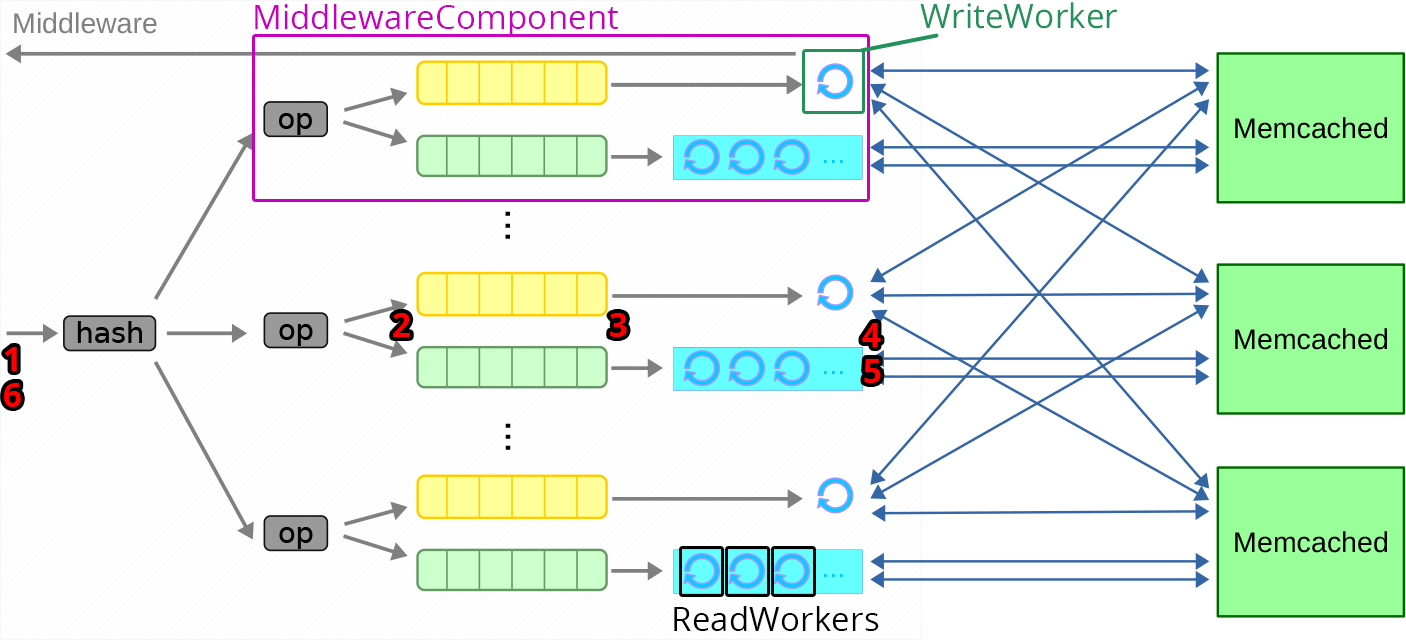
\includegraphics[width=0.8\textwidth]{figures/structure.png}
\label{fig:structure}
\end{figure}

The middleware is instrumented at six points that are also shown in Figure~\ref{fig:structure}:
\begin{enumerate}
\item $t_{created}$ -- when the request is received in \linkmain{LoadBalancer}.
\item $t_{enqueued}$ -- when the request is added to the queue.
\item $t_{dequeued}$ -- when the request is removed from the queue.
\item $t_{forwarded}$ -- when the request has been sent to all the servers (one server for GET requests and $R$ servers for SET requests).
\item $t_{received}$ -- when responses to the request have been received from all servers.
\item $t_{returned}$ -- when the response is returned to the client.
\end{enumerate}

\todo{"Shortly outline the main design decisions?"}

\subsection{Load Balancing and Hashing}\label{sec:desc:hashing}

The hashing is implemented by \linkmain{UniformHasher}. The hashing scheme for a given key s works as follows:
\begin{enumerate}
\item s is hashed into a 32-bit signed integer using Java's native \code{String.hashCode()}.
\item The hash is used to set the seed of a random number generator (\code{java.util.Random}).
\item The first random number that the generator returns is used.
\end{enumerate}

The uniformity of hashing was also validated in tests (see \linktest{UniformHasherTest}). For 1 million random strings and 13 target machines, the distribution to different machines was the following:

\begin{verbatim}
Machine   0 got      76706 hits.
Machine   1 got      76896 hits.
Machine   2 got      76718 hits.
Machine   3 got      76829 hits.
Machine   4 got      77102 hits.
Machine   5 got      76980 hits.
Machine   6 got      76467 hits.
Machine   7 got      76940 hits.
Machine   8 got      77194 hits.
Machine   9 got      76896 hits.
Machine  10 got      77107 hits.
Machine  11 got      76785 hits.
Machine  12 got      77380 hits.
\end{verbatim}

As apparent, the distribution is indeed uniform.

Selection of replicated machines for a given replication factor $R$ was done by first selecting the primary machine using the scheme described above, and then selecting the next $R-1$ machines for replication. E.g. for a setup with 8 memcached servers and $R=5$, a key whose primary machine is 5 would be replicated to machines 6, 7, 0, and 1.

\subsection{Write Operations and Replication}\label{sec:desc:writes}

The write operations are handled by \linkmain{WriteWorker}s. Each \linkmain{WriteWorker} runs on one thread and has exactly one connection to each memcached server it needs to write to, so in total $R$ connections (where $R$ is the replication factor).

\linkmain{WriteWorker} runs an infinite while-loop in which it does two distinct things.

Firstly, if there are any requests available in the queue of SET-requests, it removes one request r from the queue. It then writes to each of the replication servers without waiting for a response, i.e. it writes the whole SET-request to the first server, then to the second server, and so on. For the non-replicated case, only one request is sent.

Secondly, \linkmain{WriteWorker} checks all memcached servers to see if any of them have responded. This is done in a non-blocking manner using \code{java.nio}: if a server is not yet ready to respond, other servers will be checked. \linkmain{WriteWorker} keeps track of all responses to the same request and once all servers have returned a response, the worst out of the $R$ responses is forwarded to the client. For the non-replicated case, this process reduces to just forwarding the response from memcached to the client.


\todo{Estimate of latencies -- replicated and non-replicated}
Give an estimate of the latencies the writing operation will incur, and generalize it to the replicated case. What do you expect will limit the rate at which writes can be carried out in the system (if anything)?

\subsection{Read Operations and Thread Pool}\label{sec:desc:reads}

The read operations are handled by \href{https://gitlab.inf.ethz.ch/pungast/asl-fall16-project/blob/master/src/main/java/asl/ReadWorker.java}{ReadWorker}s. Each \linkmain{ReadWorker} runs on one thread and has exactly one socket connection to its assigned memcached server.

Every \linkmain{ReadWorker} runs an infinite while-loop in which it takes a request r from its assigned queue of GET-requests, writes the contents of r to its assigned memcached server, blocks until the response from memcached arrives, sets the response buffer of r to what it received from memcached and finally notifies \linkmain{LoadBalancer} that r is ready for returning by setting \code{r.hasResponse} to \code{true}.

Since multiple \linkmain{ReadWorkers} read from the queue of GET-requests at the same time as the \linkmain{LoadBalancer} is inserting elements, the queue needs to be safe to concurrent access by multiple threads. For this reason, \code{BlockingQueue} was chosen; in particular, the \code{ArrayBlockingQueue} subclass of \code{BlockingQueue}. The maximum size of the queue was set to a constant 200 (defined in \code{MiddlewareMain.QUEUE_SIZE}), because 3 load generating machines each with 64 concurrent clients can generate a maximum of $3 \cdot 64 = 192 < 200$ requests at a time, which in the worst (although unlikely) case will all be forwarded to the same server.


\section{Memcached Baselines}\label{sec:baseline}

\todo{}

This section will report experimental results. All such parts will start with a short description of the experimental setup. The log files should be identified by a short name, or number, which will be explicitly listed at the end of the document (see Logfile Listing at the end).  \textbf{If this table is missing or the logfiles listed can't be found in your repository the experiment could be considered invalid, and no points will be awarded!}
For baseline measurement of memcached provide \textbf{two} graphs (Section~\ref{sec:baseline:tput} and \ref{sec:baseline:rt}), one with aggregated throughput and one with average response time and standard deviation as a function of number of virtual clients. Increase these in steps from 1 to 128. Give a short explanation of memcache's behavior and find the number of virtual clients that saturate the server.

\small{
\smallskip
\begin{tabular}{|c|c|}
\hline Number of servers & 1 \\ 
\hline Number of client machines & 1 to 2 \\ 
\hline Virtual clients / machine & 1 to 64 \\ 
\hline Workload & Key 16B, Value 128B, Writes 1\% \footnotemark \\
\hline Middleware & Not present \\ 
\hline Runtime x repetitions & 30s x 5 \\ 
\hline Log files & microbench1, microbench2, \ldots \\
\hline 
\end{tabular} }

\footnotetext{As starting point use the workloads provided in \url{http://www.systems.ethz.ch/sites/default/files/file/asl2016/memaslap-workloads.tar}. Use by default the \emph{small} workload. In later experiments you can and should change read-write ratios and potentially use other value sizes.}




\subsection{Throughput}\label{sec:baseline:tput}
See previous explanation.
\subsection{Response time}\label{sec:baseline:rt}
See previous explanation.

\section{Stability Trace}\label{sec:trace}

\todo{}

In this section you will have to show that the middleware is functional and it can handle a long-running workload without crashing or degrading in performance. For this you will run it with full replication for one hour connected to three memcache instances and three load generator machines.
You will have to provide two graphs. The x-axis is time and the y-axis is either throughput or response time. Include standard deviation whenever applicable. 

\small{
\smallskip
\begin{tabular}{|c|c|}
\hline Number of servers & 3 \\ 
\hline Number of client machines & 3 \\ 
\hline Virtual clients / machine &  64 (explain if chosen otherwise) \\ 
\hline Workload & Key 16B, Value 128B, Writes 1\% (see footnote) \\
\hline Middleware & Replicate to all (R=3) \\ 
\hline Runtime x repetitions & 1h x 1 \\ 
\hline Log files & trace1, \ldots \\
\hline 
\end{tabular} }



\subsection{Throughput}
See previous explanation.

\subsection{Response time}
See previous explanation.

\subsection{Overhead of middleware}

Compare the performance you expect based on the baselines and the one you observe in the trace and quantify the overheads introduced by the middleware (if any), Look at both response time and achievable throughput when making the comparison. Provide an overview of the overheads in a table form.


\pagebreak

\section*{Logfile listing}

\begin{tabular}{|c|l|}
\hline \textbf{Short name }& \textbf{Location} \\ 
\hline microbench1 & \url{https://gitlab.inf.ethz.ch/.../baseline/logfile.log} \\ 
\hline microbench2 & \url{https://gitlab.inf.ethz.ch/.../baseline/logfile2.log} \\ 
\hline trace1 & \url{https://gitlab.inf.ethz.ch/.../baseline/logfile.log} \\ 
\hline \dots & \dots \\ 
\hline 
\end{tabular} 

\end{document}